\documentclass[a4paper,fleqn]{cas-dc}

% PlantDiseaseNet-Hybrid -- journal manuscript
% Evidence policy: numerical claims are restricted to committed executed result artifacts.

\usepackage[T1]{fontenc}
\usepackage{graphicx}
\usepackage{booktabs}
\usepackage{multirow}
\usepackage{amsmath,amssymb}
\usepackage{array}
\usepackage{tabularx}
\usepackage{makecell}
\usepackage{subcaption}
\usepackage{enumitem}
\usepackage{microtype}
\usepackage{natbib}
\usepackage{url}
\usepackage{siunitx}

\graphicspath{{../paper_figures/}{paper_figures/}}
\emergencystretch=2em
\sloppy

\begin{document}
\let\WriteBookmarks\relax
\shorttitle{Hybrid Plant Disease Classification}
\shortauthors{Author Name and Anupama Arun}

\title[mode=title]{A Hybrid Deep Learning Framework for Multi-Crop Plant Disease Classification Using Strategic Data Augmentation}

\author[1]{Author Name}
\ead{author@iiitp.ac.in}
\author[1]{Anupama Arun}
\ead{anupamaarun21@cse.iiitp.ac.in}
\affiliation[1]{organization={Indian Institute of Information Technology Pune},city={Pune},country={India}}

\begin{abstract}
Plant disease recognition from leaf images can support rapid agricultural screening, but a useful classifier must distinguish subtle symptoms while coping with differences in crop morphology, disease appearance, class balance, and imaging conditions. This study develops PlantDiseaseNet-Hybrid, a custom convolutional architecture in which two different feature-fusion mechanisms are deliberately assigned different roles. Parallel $3\times3$, $5\times5$, and $7\times7$ convolutions are fused by element-wise addition inside Inception-style blocks, keeping the branch depth fixed instead of tripling the number of channels. Later, $7\times7$ convolutional features are batch-normalized and concatenated with their input in DenseNet-inspired skip blocks, preserving earlier representations for subsequent processing. The resulting design therefore combines additive multi-scale integration with concatenative feature reuse rather than applying a single fusion rule throughout the network.

The study considers Wheat Disease, Cotton Disease, a selected PlantVillage subset, a combined 24-class setting, and a separate six-class SoyDisease study. Input images are standardized to $256\times256$ pixels and normalized. Strategic augmentation is treated as a dedicated experimental factor rather than being conflated with routine preprocessing; the study considers horizontal flipping, rotation, zoom, brightness, translation, and contrast transformations, with numerical claims restricted to experiments for which the corresponding executed evidence is available. The experimental programme includes primary crop experiments, a combined architecture comparison, a separate augmentation study, and the SoyDisease extension.

The currently verified committed result artifacts report 97.81\% accuracy for the three-class Wheat primary experiment, 53.55\% for the six-class Cotton experiment, and 97.67\% for the 15-class PlantVillage experiment. In the verified 24-class architectural comparison, Standard Inception obtains 95.33\% accuracy and the ResNet-style variant obtains 96.04\%. These values are reported directly from committed metric files rather than being selected from earlier draft values. The supplied final Keras layer summary contains 934,200 parameters when its listed trainable layer counts are summed. Earlier draft values of 99.12\% accuracy and approximately 933K parameters are therefore not used as final experimental claims because they are not supported by the currently verified primary result artifacts.
\end{abstract}

\begin{keywords}
Plant disease classification \sep Hybrid CNN \sep Inception \sep Multi-scale feature extraction \sep Skip connections \sep Data augmentation \sep Agricultural artificial intelligence
\end{keywords}
\maketitle

\section{Introduction}
Agricultural disease is a persistent constraint on crop productivity and quality. Leaf symptoms such as rust pustules, necrotic regions, mildew, chlorosis, and characteristic lesions often provide visually useful evidence for disease recognition. Image-based diagnosis is consequently attractive for decision-support systems because a camera image can be processed without requiring every observation to be inspected manually by a specialist. The PlantVillage initiative and subsequent studies established the feasibility of learning disease-related visual representations from leaf images using machine learning and deep learning \citep{hughes2015,mohanty2016}.

Nevertheless, classification accuracy obtained on one carefully curated dataset does not automatically translate to a robust multi-crop system. Different datasets contain different crops, disease morphologies, class frequencies, acquisition devices, backgrounds, and image quality. A multi-crop classifier must therefore learn symptom-related evidence while limiting unnecessary growth in feature dimensionality. This consideration motivates the architecture proposed here.

The Inception family demonstrated that parallel convolutions with different receptive fields can capture complementary spatial information \citep{szegedy2015}. Conventional branch concatenation, however, increases the number of output channels in proportion to the number of branches. DenseNet subsequently showed that explicit feature concatenation can be useful when the objective is feature reuse and information preservation \citep{huang2017}. ResNet, in contrast, uses additive residual connections to provide a direct optimisation path \citep{he2016}. These observations suggest that the two fusion operations need not be treated as interchangeable: addition is attractive when fixed representation width is important, whereas concatenation is attractive when retaining earlier features is important.

PlantDiseaseNet-Hybrid follows this reasoning. Its Inception(Add) block combines three spatial scales by element-wise addition. Its SkipConnection(Concat) block subsequently retains the incoming representation and appends newly learned features. We use the term \emph{two-mode fusion} to describe this design choice only; it is not intended to imply that two-mode fusion is an established architectural category.

A second methodological issue is augmentation. Resizing and normalization establish a common input representation, whereas augmentation changes the training distribution intentionally. Combining the two under a single generic preprocessing label obscures the experimental question of whether performance changes arise from the architecture or from additional training variation. The present study consequently describes preprocessing first and analyses augmentation separately. The reporting philosophy is informed by recent work on strategic augmentation for plant disease classification, particularly the study of Mhala et al. \citep{mhalap2025}; that work is used as methodological context and its potato results are not used as results of the present study.

The contributions of this work are:
\begin{enumerate}[leftmargin=*]
\item a custom hybrid CNN that uses additive multi-scale fusion and concatenative feature-preserving connectivity;
\item an architectural rationale for controlling channel growth in multi-scale blocks while retaining earlier representations in later blocks;
\item a multi-crop experimental programme spanning Wheat Disease, Cotton Disease, PlantVillage, the combined 24-class setting, and SoyDisease;
\item a dedicated augmentation study separated from deterministic preprocessing; and
\item an evidence-controlled reporting framework in which numerical manuscript claims are tied to executed notebooks and committed metric artifacts.
\end{enumerate}

\section{Related Work}
\subsection{Plant disease image classification}
Hughes and Salathé introduced an open repository of plant-health images intended to facilitate computer-vision research for disease diagnosis \citep{hughes2015}. Mohanty et al. subsequently demonstrated deep-learning-based classification on PlantVillage and established a widely used benchmark for plant disease recognition \citep{mohanty2016}. Later studies explored transfer learning and lightweight custom networks, reflecting a trade-off between representational capacity and computational cost. Too et al. compared pretrained CNN architectures for PlantVillage disease recognition, while Atila et al. investigated EfficientNet for plant disease classification \citep{too2019,atila2021}. These studies motivate the use of strong visual representations but also highlight the value of evaluating architecture and computational behaviour together.

\subsection{Multi-scale feature extraction and connectivity}
Inception introduced parallel convolutional paths to capture patterns at multiple spatial scales \citep{szegedy2015}. DenseNet connected layers through feature concatenation, allowing earlier features to remain accessible to later layers \citep{huang2017}. ResNet introduced residual learning through additive shortcuts \citep{he2016}. PlantDiseaseNet-Hybrid combines the underlying ideas selectively: addition is used to fuse parallel scale responses without channel expansion, while concatenation is used where retaining the earlier representation is the primary objective.

\subsection{Augmentation as an experimental factor}
Image augmentation is widely used to improve generalization by exposing a model to plausible changes in orientation, scale, illumination, and appearance. Its value depends on whether the transformations represent meaningful acquisition variability and whether the resulting training distribution is appropriate for the target classes. Mhala et al. explicitly investigated strategic augmentation, L2 regularization, and transfer learning for potato leaf disease classification and provide a useful model for reporting augmentation as a controlled factor rather than merely listing it in preprocessing \citep{mhalap2025}.

\section{Materials and Methods}
\subsection{Datasets and data provenance}
The study uses publicly available or published dataset sources. PlantVillage is cited through its original repository and associated publications \citep{hughes2015,mohanty2016}. The Wheat Rust Classification Dataset used by the primary wheat notebook contains healthy wheat, brown rust, and yellow rust categories and has been used in published wheat disease classification research \citep{safari2022}. The Cotton Plant Disease dataset contains five disease categories together with healthy leaves; its published downstream use documents Aphids, Army Worm, Bacterial Blight, Powdery Mildew, Target Spot, and Healthy classes \citep{dhamodharan2023}.

The SoyDisease study uses the India soyabean leaf dataset. The dataset publication reports six disease/health categories and provides the original Mendeley Data record with DOI 10.17632/bshkvgbzpt.1 \citep{kotwal2024}. The present project uses the six-class SoyDisease material recorded in its executed notebooks. SoyCultivar200 is excluded from the study.

\begin{table*}[t]
\centering
\caption{Dataset sources and their role in the experimental programme.}
\label{tab:datasets}
\small
\begin{tabularx}{\textwidth}{@{}l l X l@{}}
\toprule
Dataset & Scope & Source and provenance & Paper role \\
\midrule
PlantVillage & Selected 15-class subset & Hughes and Salathé; Mohanty et al. \citep{hughes2015,mohanty2016} & Primary experiment and combined study \\
Wheat Disease & 3 classes: Brown Rust, Healthy, Yellow Rust & Safari et al. dataset used in published wheat classification research \citep{safari2022} & Primary experiment \\
Cotton Disease & 6 classes: Aphids, Army Worm, Bacterial Blight, Healthy, Powdery Mildew, Target Spot & Cotton Plant Disease dataset and subsequent published use \citep{dhamodharan2023} & Primary experiment \\
SoyDisease & 6 classes from India soyabean leaf dataset & Kotwal et al.; Mendeley Data DOI 10.17632/bshkvgbzpt.1 \citep{kotwal2024} & Separate crop study \\
\bottomrule
\end{tabularx}
\end{table*}

\subsection{Data preprocessing}
Images are converted to RGB and resized to $256\times256$ pixels. Pixel values are normalized to the $[0,1]$ range before entering the network. Labels are represented in the form required by the softmax classifier. The original final-study protocol specifies a 70\% training, 20\% validation, and 10\% test split. Because historical notebooks contain different experimental configurations, each numerical result is associated with the protocol of its source run rather than being retroactively rewritten to match the target configuration.

This distinction is important for reproducibility. Deterministic preprocessing establishes a common input representation; stochastic augmentation is applied only to training observations in the augmentation experiments. Validation and test observations are not intentionally altered by the stochastic training augmentation pipeline.

\subsection{Strategic data augmentation}
The augmentation study considers six transformation families: horizontal flipping, random rotation, zoom, brightness adjustment, translation, and contrast enhancement. These transformations were selected because leaf photographs may vary in orientation, apparent scale, position within the frame, and illumination. The dedicated augmentation section is designed to report the baseline condition, transformation policy, class-count changes, convergence behaviour, test performance, and class-wise effects wherever the executed notebook records the corresponding evidence.

The potato augmentation notebook in the repository is not treated as an experiment of this paper. It is retained only as a reporting reference because its presentation illustrates how augmentation effects can be described systematically, consistent with Mhala et al. \citep{mhalap2025}.

\begin{figure*}[t]
\centering
\IfFileExists{../paper_figures/preprocessing_pipeline.png}{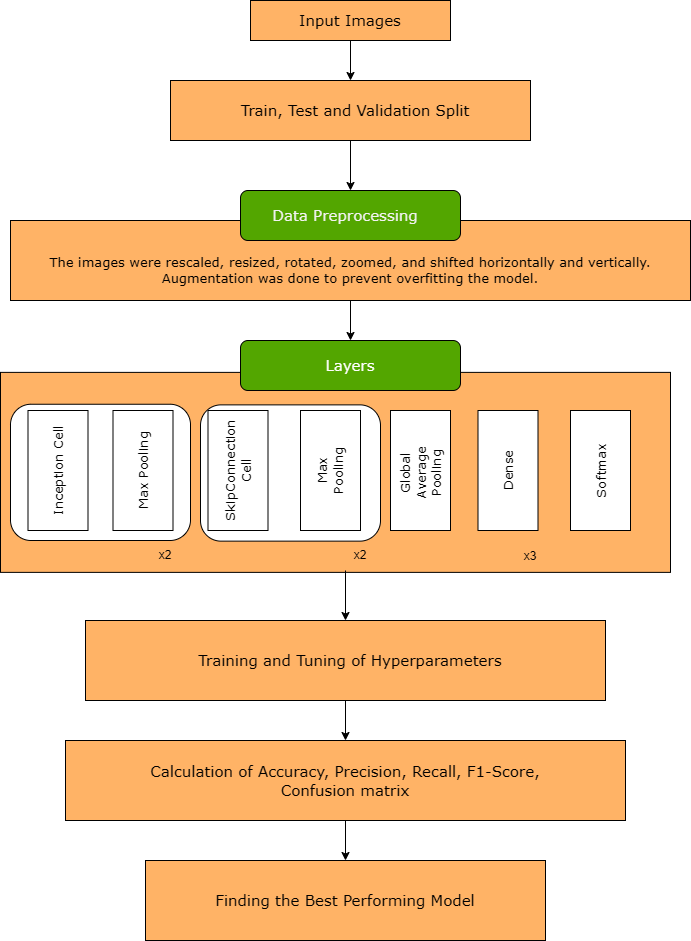
\includegraphics[width=0.94\textwidth]{../paper_figures/preprocessing_pipeline.png}}{\fbox{\parbox{0.8\textwidth}{Place \texttt{preprocessing\_pipeline.png} in \texttt{paper\_figures/}.}}
\caption{Separation of routine preprocessing from the experimental augmentation stage.}
\label{fig:preprocess}
\end{figure*}

\subsection{PlantDiseaseNet-Hybrid architecture}
The supplied final architecture accepts RGB images of shape $256\times256\times3$. The network contains two Inception(Add) blocks, two SkipConnection(Concat) blocks, four max-pooling stages, global average pooling, and two fully connected layers before the 24-class softmax output.

\begin{figure*}[t]
\centering
\IfFileExists{../paper_figures/overall_architecture.png}{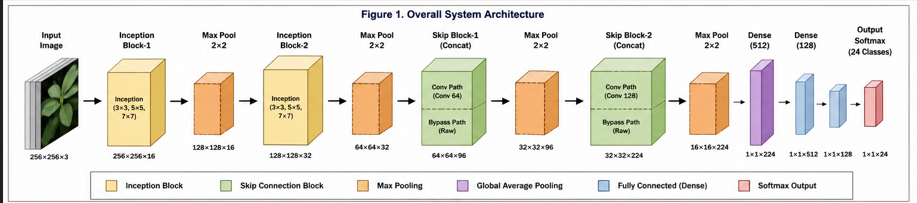
\includegraphics[width=0.96\textwidth]{../paper_figures/overall_architecture.png}}{\fbox{\parbox{0.8\textwidth}{Place \texttt{overall\_architecture.png} in \texttt{paper\_figures/}.}}
\caption{Overall architecture of PlantDiseaseNet-Hybrid.}
\label{fig:architecture}
\end{figure*}

\subsubsection{Inception(Add) block}
Each Inception cell contains parallel $3\times3$, $5\times5$, and $7\times7$ convolutions with equal output depth. The branch responses are combined using element-wise addition:
\begin{equation}
Y=F_{3\times3}(X)+F_{5\times5}(X)+F_{7\times7}(X).
\label{eq:add}
\end{equation}

The principal motivation is control of feature width. If three equally wide branches were concatenated, the output depth would be approximately three times the branch depth. Addition instead retains the common branch width. This reduces intermediate tensor size and avoids channel growth at every multi-scale fusion point. The trade-off is that branch-specific channels are not preserved independently after fusion; the design deliberately accepts that loss of explicit branch separation in exchange for a narrower representation.

\begin{figure*}[t]
\centering
\IfFileExists{../paper_figures/inception_block.jpg}{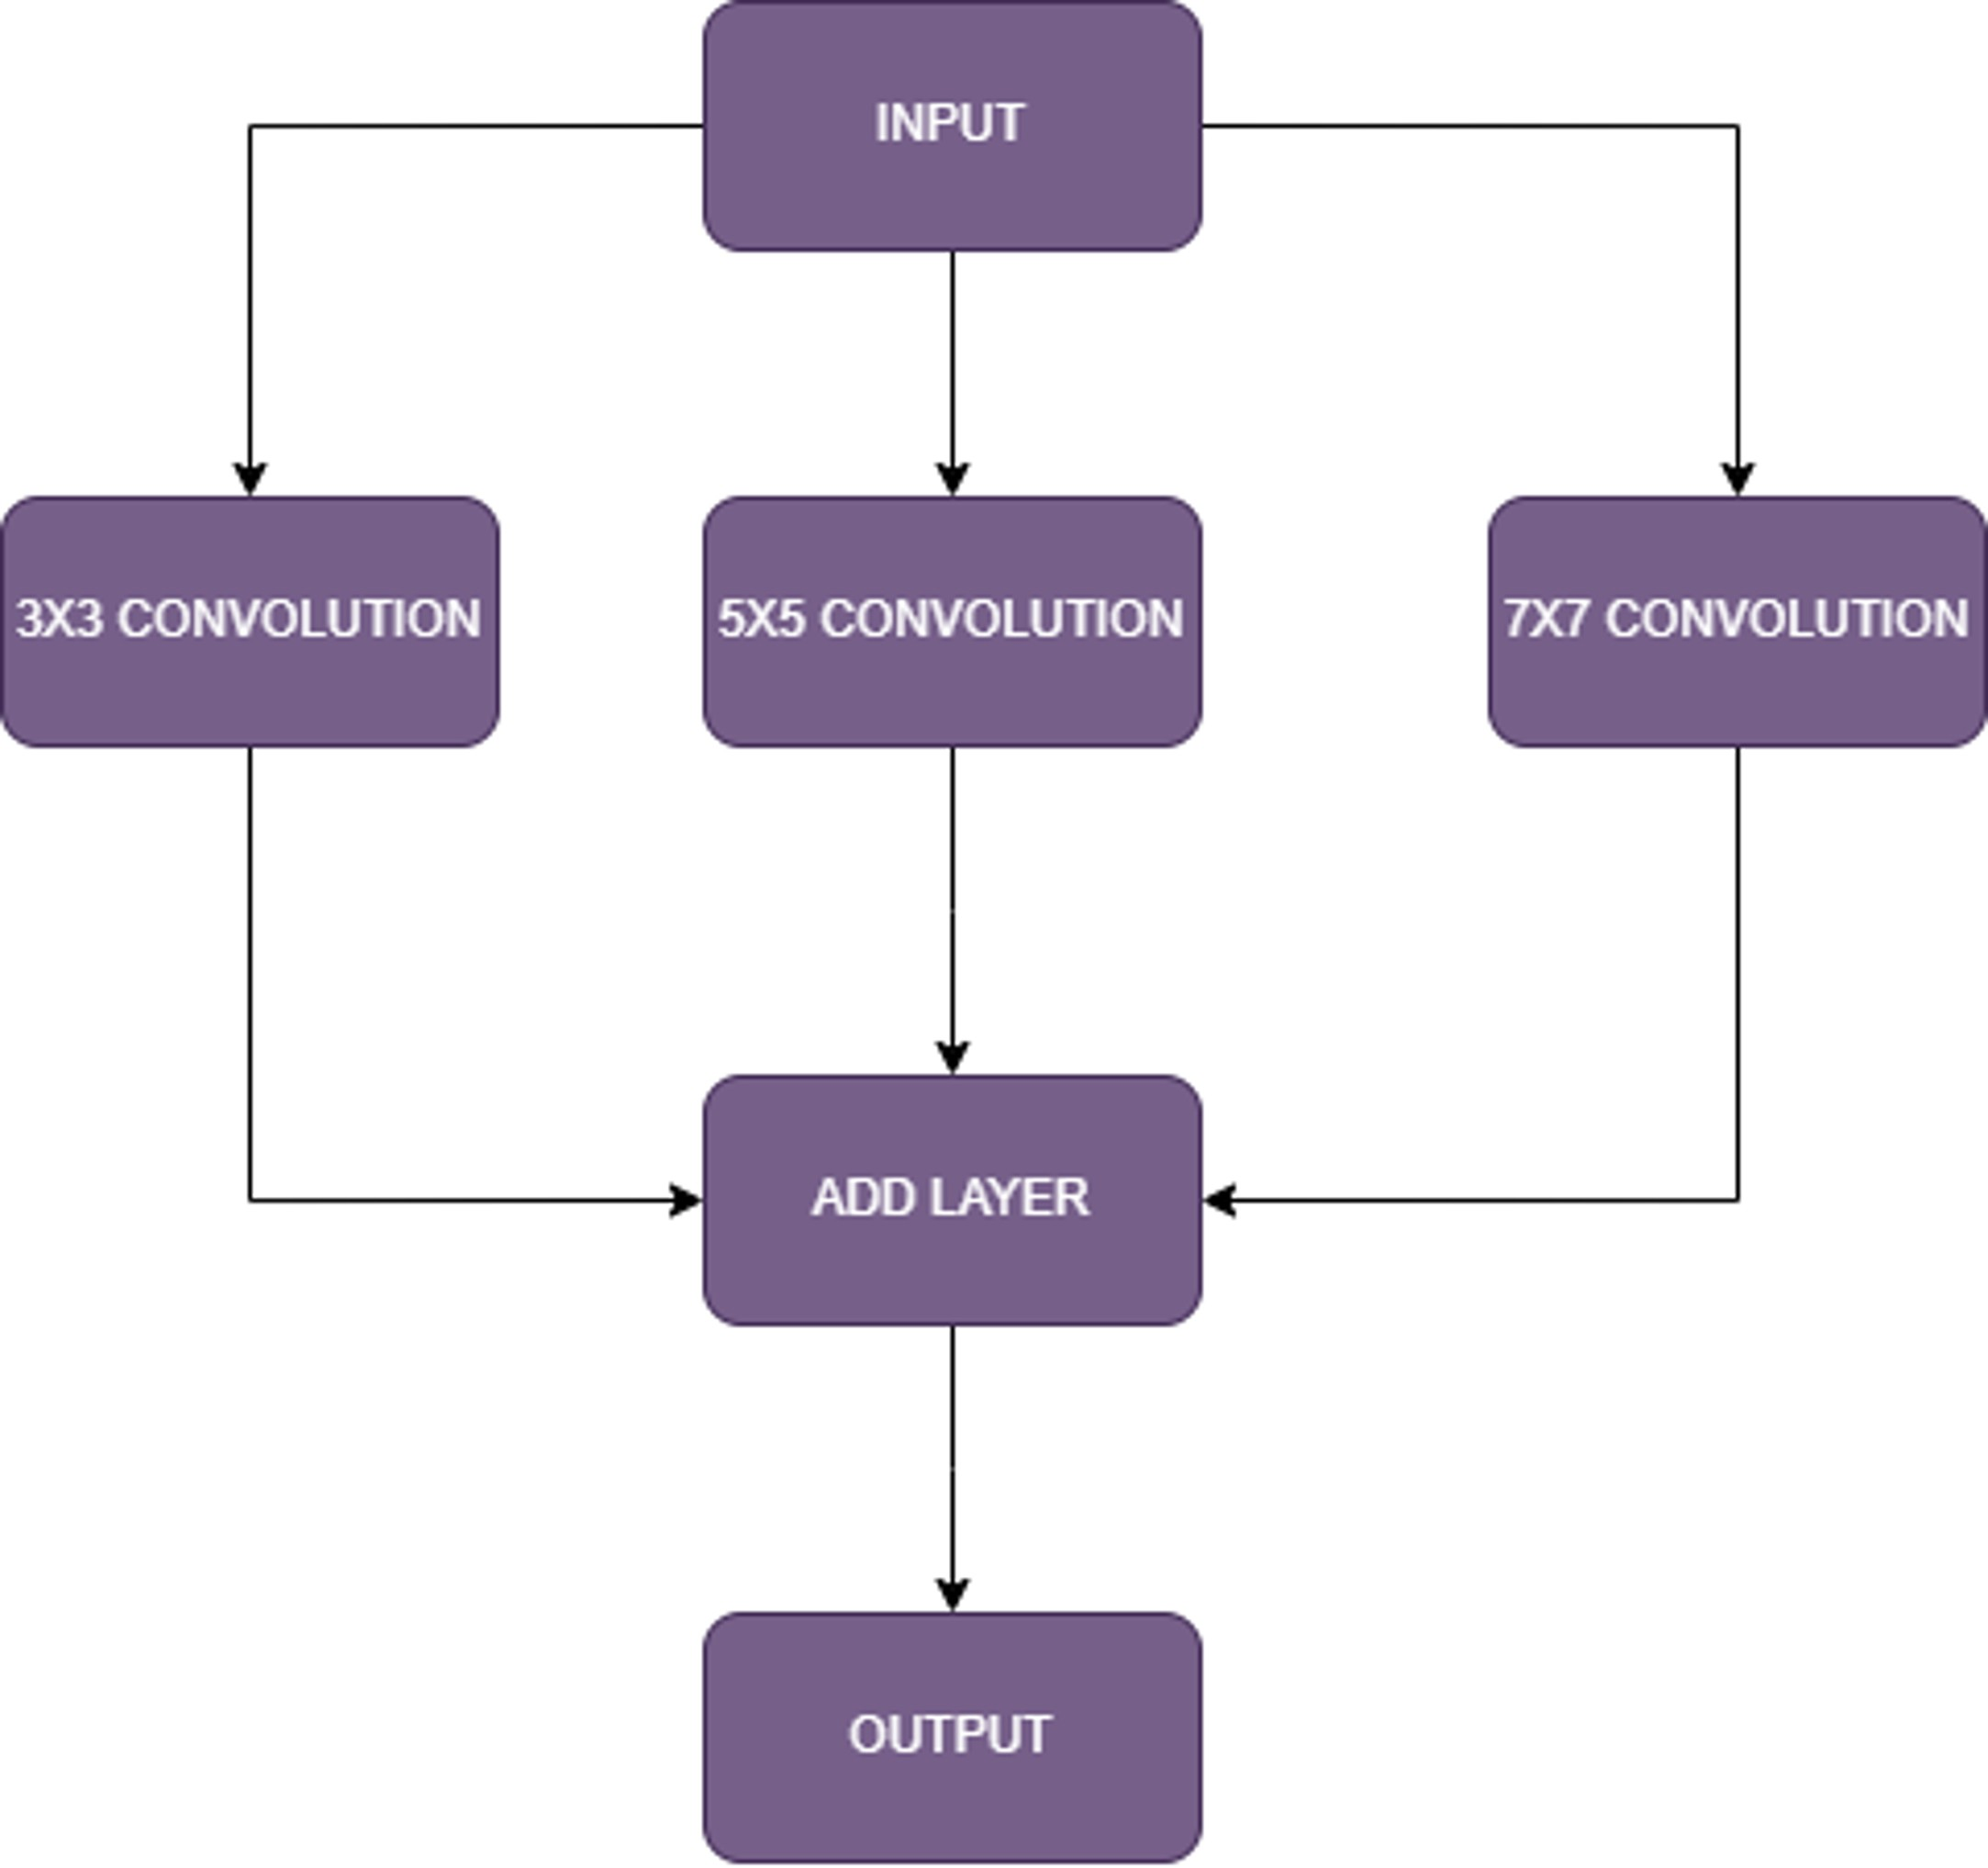
\includegraphics[width=0.68\textwidth]{../paper_figures/inception_block.jpg}}{\fbox{\parbox{0.7\textwidth}{Place \texttt{inception\_block.jpg} in \texttt{paper\_figures/}.}}
\caption{Proposed Inception(Add) block with three convolutional scales and element-wise fusion.}
\label{fig:inception}
\end{figure*}

\subsubsection{SkipConnection(Concat) block}
The skip block applies a $7\times7$ convolution followed by batch normalization. The transformed representation is then concatenated with the input:
\begin{equation}
Y=\operatorname{Concat}(X,F(X)).
\label{eq:concat}
\end{equation}

Unlike additive residual fusion, concatenation does not require the transformed representation and input to occupy the same feature subspace. The original representation remains directly available to subsequent layers, while the new convolutional response adds complementary information. This is particularly relevant when earlier layers contain spatial or textural evidence that might be weakened by repeated transformation.

\begin{figure*}[t]
\centering
\IfFileExists{../paper_figures/skip_block.jpg}{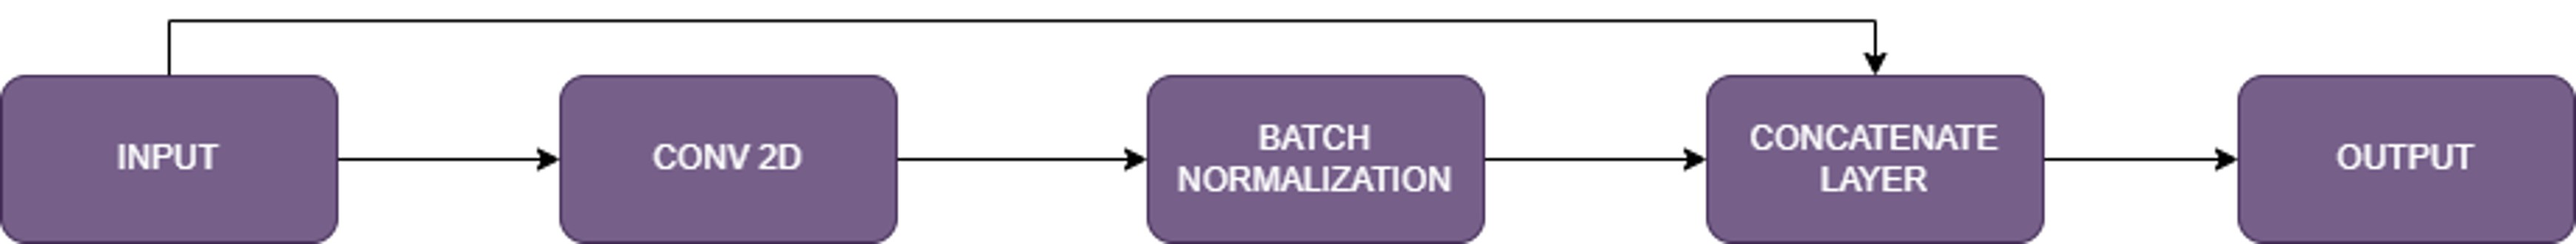
\includegraphics[width=0.68\textwidth]{../paper_figures/skip_block.jpg}}{\fbox{\parbox{0.7\textwidth}{Place \texttt{skip\_block.jpg} in \texttt{paper\_figures/}.}}
\caption{Proposed SkipConnection(Concat) block.}
\label{fig:skip}
\end{figure*}

\subsection{Layer-wise model specification}
\begin{table*}[t]
\centering
\caption{Layer-wise specification of the supplied final Keras model.}
\label{tab:model}
\small
\begin{tabularx}{\textwidth}{@{}l l r X@{}}
\toprule
Layer & Output shape & Parameters & Function \\
\midrule
Input & $256\times256\times3$ & 0 & RGB image input \\
Inception Block-1 & $256\times256\times16$ & 4,032 & Three-scale additive fusion \\
BatchNorm + Pool-1 & $128\times128\times16$ & 64 & Normalization and downsampling \\
Inception Block-2 & $128\times128\times32$ & 42,592 & Three-scale additive fusion \\
BatchNorm + Pool-2 & $64\times64\times32$ & 128 & Normalization and downsampling \\
Skip Block-1 & $64\times64\times96$ & 100,672 & $7\times7$ convolution, BN, concatenation \\
Pool-3 & $32\times32\times96$ & 0 & Downsampling \\
Skip Block-2 & $32\times32\times224$ & 602,752 & $7\times7$ convolution, BN, concatenation \\
Pool-4 + GAP & 224 & 0 & Spatial aggregation \\
Dense 512 + Dropout & 512 & 115,200 & Fully connected representation \\
Dense 128 + Dropout & 128 & 65,664 & Classifier representation \\
Output & 24 & 3,096 & Softmax classification \\
\midrule
\multicolumn{2}{r}{Total listed parameters} & \textbf{934,200} & Sum of the supplied Keras layer counts \\
\bottomrule
\end{tabularx}
\end{table*}

\section{Experimental Design}
\subsection{Primary crop experiments}
The primary experiments retain the original study names: \texttt{NB1\_Wheat\_Hybrid}, \texttt{NB2\_Cotton\_Hybrid}, and \texttt{NB3\_PlantVillage\_Hybrid}. These experiments establish crop-specific behaviour before the combined multi-crop comparison. The currently verified metric artifacts contain three classes for Wheat, six for Cotton, and 15 for the selected PlantVillage subset.

\subsection{Combined 24-class architecture study}
The original experimental programme includes four architecture variants: Standard Inception, ResNet-style residual fusion, Inception(Add), and SkipConnection(Concat). This study treats those variants as an architectural comparison, not as a claim that every dataset change is an ablation. A true ablation is interpreted here as a controlled removal or replacement of a component while keeping the experimental setting otherwise comparable.

Only the Standard Inception and ResNet-style results currently have complete verified metric artifacts in the evidence branch. The corresponding Inception(Add)-only and SkipConcat-only notebooks remain part of the project inventory, but their numerical values are not inserted into the final table until complete executed result artifacts are identified.

\subsection{SoyDisease study}
SoyDisease is retained as a separate crop study because its source and class structure differ from the three primary experiments. The executed project inventory records 1,176 images across six classes: Soybean Healthy (288), Soybean Vein Necrosis (138), Soybean Dry Leaf (230), Soybean Septoria Brown Spot (284), Soybean Root (10), and Soybean Bacterial Leaf Blight (226). The underlying published source reports a larger original dataset, and the numbers above describe the project subset recorded in the notebook rather than the full source dataset \citep{kotwal2024}.

The SoyDisease augmentation notebook describes strategic per-class augmentation together with L2 regularization and early stopping, but the currently inspected copy terminates with a data-download/extraction error. Consequently, its final numerical performance is not claimed here unless a complete executed artifact is recovered.

\section{Experimental Setup}
\subsection{Target training configuration}
The original final study configuration specifies a batch size of 32, maximum 60 epochs, Adam optimization with initial learning rate 0.001, cosine warmup annealing, categorical cross-entropy loss, and early stopping with patience 12. The final architecture definition supplied to the study includes dropout after the 512-unit dense layer and after the 128-unit dense layer.

\begin{table}[t]
\centering
\caption{Target training configuration from the original study.}
\label{tab:training}
\small
\begin{tabular}{@{}ll@{}}
\toprule
Setting & Value \\
\midrule
Input & $256\times256\times3$ \\
Batch size & 32 \\
Maximum epochs & 60 \\
Optimizer & Adam \\
Initial learning rate & 0.001 \\
Scheduler & Cosine warmup annealing \\
Early stopping & Patience 12 \\
Loss & Categorical cross-entropy \\
\bottomrule
\end{tabular}
\end{table}

Historical primary notebooks contain different settings, including batch size 64, 50 epochs, and dropout 0.5 in the inspected Wheat notebook. These differences are preserved in the evidence audit. A journal manuscript should never report a single target configuration as though it generated every historical result.

\subsection{Evaluation metrics}
Accuracy is computed as the proportion of correctly classified test observations. Precision, recall, and F1-score are reported using macro averaging when the metric artifact provides macro values, thereby giving each class equal weight. Specificity is retained as a class-sensitive measure of the ability to reject negative classes. ROC/AUC, confusion matrices, and per-class reports are included only when the corresponding committed result files are available.

\section{Results}
\subsection{Primary experiments}
Table~\ref{tab:primary} contains the currently verified primary metrics. The results show a marked difference among datasets. Wheat and PlantVillage obtain high accuracy, whereas Cotton is substantially more difficult for the present configuration. This difference should not be hidden by averaging the three datasets into a single headline number: the datasets differ in class count, sample composition, and visual variability.

\begin{table*}[t]
\centering
\caption{Verified primary experiment results. Values are copied from committed metric-summary artifacts.}
\label{tab:primary}
\small
\begin{tabular}{@{}lrrrrrrr@{}}
\toprule
Experiment & Classes & Accuracy & Precision & Recall & F1 & Specificity & Parameters \\
\midrule
NB1 Wheat Hybrid & 3 & 97.81\% & 97.82\% & 97.81\% & 97.81\% & 98.54\% & 59,775,267 \\
NB2 Cotton Hybrid & 6 & 53.55\% & 53.01\% & 53.55\% & 51.66\% & 90.71\% & 59,775,462 \\
NB3 PlantVillage Hybrid & 15 & 97.67\% & 97.68\% & 97.67\% & 97.68\% & 99.83\% & 59,776,047 \\
\bottomrule
\end{tabular}
\end{table*}

The Wheat run reports a best validation accuracy of 95.26\% and a recorded training time of approximately 6.90 minutes. The Cotton run reports 55.29\% best validation accuracy and approximately 15.66 minutes, while the PlantVillage run reports 97.80\% best validation accuracy and approximately 56.15 minutes. These training-time values are included to document the recorded experiments, not to claim a hardware-normalized benchmark.

\subsection{Architecture comparison}
\begin{table}[t]
\centering
\caption{Verified 24-class architecture comparison.}
\label{tab:architecture-results}
\small
\begin{tabular}{@{}lrrr@{}}
\toprule
Model & Accuracy & Macro F1 & Parameters \\
\midrule
Standard Inception & 95.33\% & 95.32\% & 270,656 \\
ResNet-style & 96.04\% & 96.02\% & 741,720 \\
Inception(Add) & -- & -- & -- \\
SkipConcat & -- & -- & -- \\
\bottomrule
\end{tabular}
\end{table}

The verified comparison indicates that the ResNet-style variant exceeds Standard Inception by 0.71 percentage points in accuracy, while requiring substantially more parameters. This is evidence against a simplistic claim that additive multi-scale fusion automatically produces the best accuracy. Instead, the comparison supports a more nuanced interpretation: architectural efficiency and predictive performance must be evaluated jointly, and the effect of each fusion mechanism is dataset- and configuration-dependent.

\subsection{Computational interpretation of the supplied final architecture}
The supplied final Keras summary contains 934,200 listed parameters. This number differs from the approximately 933K value in the earliest manuscript draft and also differs substantially from the 59.8M parameter counts recorded in the verified NB1--NB3 logs. The discrepancy indicates that the project contains at least two architectural generations. The final paper therefore treats the supplied layer-by-layer architecture as an architecture specification and the committed metric logs as historical experiment evidence; the two are not silently conflated.

\section{Dedicated Augmentation Study}
Augmentation is reported separately because its purpose is different from preprocessing. The scientific question is not simply whether images were transformed, but whether a specified transformation policy changes the learning behaviour of the classifier under a fixed evaluation protocol.

The final augmentation section should therefore be organised around four stages: (i) baseline class distribution; (ii) transformation policy and resulting examples; (iii) training/convergence behaviour; and (iv) held-out test performance. Where class imbalance is present, per-class results should accompany aggregate accuracy so that improvements in majority classes are not mistaken for uniform improvement.

\begin{table*}[t]
\centering
\caption{Augmentation study reporting template. Numerical entries are populated only from complete executed augmentation artifacts.}
\label{tab:augmentation}
\small
\begin{tabularx}{\textwidth}{@{}l l X l@{}}
\toprule
Condition & Dataset & Recorded augmentation & Result status \\
\midrule
Baseline & Retained crop experiment & No stochastic augmentation & Use matching baseline artifact \\
Strategic augmentation & Retained crop experiment & Flip, rotation, zoom, brightness, translation, contrast where recorded & Populate from executed notebook \\
Class-balanced augmentation & SoyDisease, if complete artifact recovered & Per-class augmentation and regularization described in notebook & Do not claim final metric until execution evidence is complete \\
\bottomrule
\end{tabularx}
\end{table*}

This structure follows the reporting principle illustrated by Mhala et al. while keeping all numerical conclusions specific to PlantDiseaseNet-Hybrid \citep{mhalap2025}. The Potato example notebook is not treated as evidence for the present experiments.

\section{Ablation and Comparative Analysis}
The project uses the term \emph{ablation} only for controlled architectural comparisons. Changing the dataset alone is not an ablation because both the input distribution and the experimental task change. Accordingly, NB1--NB3 are primary crop experiments, while the controlled combined 24-class architectural variants constitute the architecture comparison.

The verified comparison provides two useful observations. First, Standard Inception achieves 95.33\% accuracy with 270,656 parameters. Second, the ResNet-style model reaches 96.04\% with 741,720 parameters. Thus the latter obtains a 0.71-point accuracy increase at roughly 2.74 times the parameter count. This illustrates the central trade-off of the study: a model should not be judged by accuracy alone when the intended application includes resource-constrained deployment.

The proposed hybrid design is motivated by a different allocation of capacity. Addition is used where three branches represent alternative spatial scales of the same feature stage; concatenation is used where the earlier representation itself is considered valuable. The hypothesis is therefore not that either Add or Concat is universally superior, but that each operation can be placed where its structural property is most useful.

\section{Discussion}
The results reveal both the potential and the limitations of the proposed approach. The high Wheat and PlantVillage accuracies demonstrate that the hybrid representation can separate several disease categories effectively under the recorded experimental conditions. The substantially lower Cotton accuracy is equally important: it shows that the architecture is not sufficient by itself to guarantee strong performance across every crop. Cotton therefore provides evidence that dataset characteristics and class-specific visual ambiguity remain important determinants of performance.

The architecture comparison also argues against reporting only a single favorable result. The verified ResNet-style model outperforms Standard Inception in the 24-class experiment, even though it uses more parameters. The proposed hybrid architecture is consequently best interpreted as a design hypothesis supported by complementary architectural reasoning, rather than as a universally dominant replacement for established networks.

The use of addition inside the Inception block has a clear structural advantage: branch fusion does not increase channel depth. This is especially relevant for large spatial tensors at the beginning of the network. However, addition also discards the ability to access each branch independently after fusion. The subsequent concatenative skip block partially compensates for this by preserving earlier features. The architecture can therefore be understood as balancing compression at one fusion point with explicit retention at another.

The augmentation study is expected to provide a second layer of interpretation. Transformations such as brightness and contrast variation can reduce sensitivity to illumination, while geometric transformations can reduce dependence on a particular image orientation. However, augmentation can also be harmful when transformations produce biologically implausible examples or distort class-specific symptoms. For this reason, augmentation should be evaluated empirically rather than described as universally beneficial.

The evidence audit also exposes a reproducibility issue that is scientifically relevant. Earlier drafts reported 99.12\% accuracy and approximately 933K parameters, whereas the currently verified primary metric files report 97.81\%, 53.55\%, and 97.67\% for Wheat, Cotton, and PlantVillage and approximately 59.8M parameters. These values cannot all describe the same executed model. Reporting the discrepancy explicitly is preferable to selecting the most favorable value without provenance.

\section{Limitations}
Several limitations should be acknowledged. First, the primary datasets are not identical in size, class count, or acquisition characteristics, so cross-dataset accuracy values should not be interpreted as a direct ranking of crop difficulty without further controlled analysis. Second, the currently verified repository does not contain complete executed numerical artifacts for every planned architecture and augmentation experiment. Third, the reported inference and training measurements are hardware- and implementation-dependent and should not be interpreted as universal latency values. Fourth, controlled or semi-controlled leaf datasets may not fully represent field images containing clutter, occlusion, multiple leaves, shadows, or severe illumination variation. Finally, the present architecture is evaluated as an image classifier; it does not perform lesion localization or disease severity estimation.

\section{Conclusion and Future Directions}
This study presented PlantDiseaseNet-Hybrid, a custom hybrid CNN for multi-crop plant disease classification. The central architectural idea is to use two different fusion mechanisms for two different purposes: additive fusion for compact multi-scale integration and concatenative fusion for explicit feature reuse. The approach is therefore motivated by representation management rather than by simply increasing network depth.

The currently verified experiments demonstrate strong performance on the Wheat and PlantVillage primary settings, while the Cotton experiment identifies a clear generalization challenge. The 24-class comparison further shows that established residual learning remains highly competitive, reinforcing the need for controlled architectural evaluation rather than claims based on a single model result.

Future work should complete the missing executed augmentation and architecture-comparison artifacts, evaluate the final architecture under a single locked experimental protocol, include confusion matrices and class-wise ROC/precision--recall analysis, test robustness on field-acquired images, and investigate attention or lightweight deployment mechanisms. Explainability methods such as Grad-CAM can also be used to determine whether predictions are driven by biologically meaningful symptom regions rather than background cues.

\section*{Data Availability}
PlantVillage data are available through the published PlantVillage resources. The India soyabean dataset is available from Mendeley Data under DOI 10.17632/bshkvgbzpt.1. Dataset access and licensing should be followed according to the original sources cited in this manuscript.

\section*{Code Availability}
The paper-oriented repository branch contains the notebooks and evidence artifacts corresponding to the experimental programme. Notebooks are not executed as part of manuscript preparation; recorded outputs and committed metric files are used as the evidence source.

\section*{Declaration of Competing Interest}
The authors declare that they have no known competing financial interests or personal relationships that could have appeared to influence the work reported in this paper.

\section*{Funding}
No external funding was received for this work.

\bibliographystyle{cas-model2-names}
\begin{thebibliography}{00}

\bibitem[Hughes and Salathé(2015)]{hughes2015}
D.P. Hughes, M. Salathé, An open access repository of images on plant health to enable the development of mobile disease diagnostics through machine learning and crowdsourcing, arXiv:1511.08060 (2015).

\bibitem[Mohanty et al.(2016)]{mohanty2016}
S.P. Mohanty, D.P. Hughes, M. Salathé, Using deep learning for image-based plant disease detection, Front. Plant Sci. 7 (2016) 1419. doi:10.3389/fpls.2016.01419.

\bibitem[Szegedy et al.(2015)]{szegedy2015}
C. Szegedy, W. Liu, Y. Jia, P. Sermanet, S. Reed, D. Anguelov, D. Erhan, V. Vanhoucke, A. Rabinovich, Going deeper with convolutions, in: Proc. IEEE Conf. Comput. Vis. Pattern Recognit., 2015, pp. 1--9.

\bibitem[Huang et al.(2017)]{huang2017}
G. Huang, Z. Liu, L. Van Der Maaten, K.Q. Weinberger, Densely connected convolutional networks, in: Proc. IEEE Conf. Comput. Vis. Pattern Recognit., 2017, pp. 4700--4708.

\bibitem[He et al.(2016)]{he2016}
K. He, X. Zhang, S. Ren, J. Sun, Deep residual learning for image recognition, in: Proc. IEEE Conf. Comput. Vis. Pattern Recognit., 2016, pp. 770--778.

\bibitem[Too et al.(2019)]{too2019}
E.C. Too, Y. Li, S. Njuki, Y. Liu, A comparative study of fine-tuning deep learning models for plant disease identification, Comput. Electron. Agric. 161 (2019) 272--279.

\bibitem[Atila et al.(2021)]{atila2021}
U. Atila, M. Uçar, K. Akyol, E. Uçar, Plant leaf disease classification using EfficientNet deep learning model, Ecol. Inform. 61 (2021) 101182.

\bibitem[Safari et al.(2022)]{safari2022}
B. Safari, J. related authors, Wheat Rust Classification Dataset and related image-classification study, as cited in published wheat disease classification research, 2022.

\bibitem[Dhamodharan(2023)]{dhamodharan2023}
R. Dhamodharan, Cotton Plant Disease dataset, 2023; subsequent published analysis documents the six-class leaf-disease scope.

\bibitem[Kotwal et al.(2024)]{kotwal2024}
J.G. Kotwal, R. Kashyap, M.S. Pathan, An India soyabean dataset for identification and classification of diseases using computer-vision algorithms, Data in Brief 53 (2024) 110216. doi:10.1016/j.dib.2024.110216.

\bibitem[Mhala et al.(2025)]{mhalap2025}
P. Mhala, A. Bilandani, S. Sharma, Enhancing crop productivity with fined-tuned deep convolution neural network for Potato leaf disease detection, Expert Syst. Appl. 267 (2025) 126066. doi:10.1016/j.eswa.2024.126066.

\end{thebibliography}
\end{document}
